\section{Statistical criticism for VAEs}\label{sec:approach}

% \begin{figure}
%     \centering
%     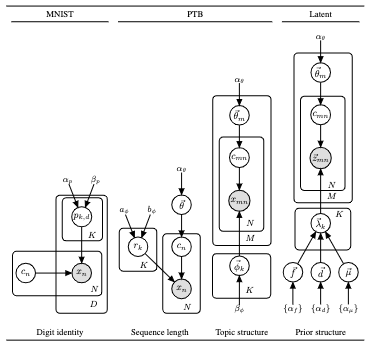
\includegraphics[width=0.5\textwidth]{sections/test.png}
%     \caption{Caption}
%     \label{fig:my_label}
% \end{figure}


% \wanote{Here we talk about the strategy for statistical criticism of VAEs, explain the role of BDA models, design the statistics by which we criticise the model (the different forms of surprisal and the different control groups) along all aspects identified earlier, explain how BDA models can be themselves checked, and explain how we generate quantitative summaries (eg, KL). }

% 1. `choose a statistic' becomes `choose a latent structure model' (e.g., naive Bayes classifier, LDA, etc); 
% 2. `compute the statistic for data/model samples' becomes `assess the surprisal of data/model samples under this model' (this is a scalar statistic);
% 3. `compute a p-value` becomes `assess the discrepancy between surprisal distributions for different groups relative to a control group'; 
% 4. we design control groups to shed light onto the fit of $p_X$ to $q_X$, the fit of $q_Z$ to $p_Z$, qualitative properties of the map between $Z$ and $X$ (\wanote{anything else?});
% 5. finally, we discuss and propose techniques to visualise and quantify discrepancies.

% \wanote{Perhaps a diagram showing something like: $D_X$ $\to$ latent structure model $\mathcal S$; then data/model samples and control groups go into $\mathcal S$ and we get surprisals; then we visualise/quantify discrepancies.}


% Interlude: we `check' or `criticise' the latent structure model itself, as well as our choice of mechanism to analyse surprisal data.

% --



%Criticising VAEs involves criticism of multiple components along multiple dimensions of practical interest.
% something on the various components? the various models we may be comparing? the various dimensions ?
%At the very least, a single VAE involves two probability distributions ($q_{ZX}$ and $p_{XZ}$), but more often than not
Our approach to comparing multiple VAEs is based on statistical criticism through Bayesian estimation \citep{kruschke2013bayesian,benavoli2017time}. We observe measurements from different groups of interest (\ie, relevant statistics of data  and/or model samples), some of which serve as control groups to help establish degrees of reasonable variation. We posit a hierarchical model of all grouped measurements and infer a posterior distribution over its latent parameters. We then use the posterior distribution to visualise and/or quantify degrees of discrepancy between any model group and a control group, and use such summaries to, for example, order model groups in terms of resemblance to the control group.
We have three criteria along which we criticise VAEs, namely,
\enumone `does $p_{X}$ fit the data?', \enumtwo `is $p_{Z|X=x}$ practically useful', \enumthree `do $p_{XZ}$ and $q_{ZX}$ offer two views of the same probability space?'. Next, we describe our approach to comparing VAEs along these three dimensions.

\paragraph{Strategy.} To criticise VAEs along criterion \enumone we compare how a real-valued statistic $T(X)$ distributes as a function of data samples $x \sim q_X$ or model samples obtained by chaining the prior and the observational model ($\hat x \sim p_{X|Z=z}$ with $z \sim p_Z$). If $T(X)$ and $T(\hat X)$ distribute similarly, then the VAEs correlate the variates in $X$ at least in the way $T(\cdot)$ does.
For criterion \enumtwo, we design a conditional statistic $T(X'|X)$ which has a structured view of $(X,X')$ and compare how it distributes as a function of data samples $x' \sim q_X$ or model samples obtained by chaining the inference model and the observational model ($\tilde x \sim p_{X|Z=z}$ with $z \sim q_{Z|X=x}$) given a seed data sample $x \sim q_X$. If $T(X'|X)$ and $T(\tilde X|X)$ distribute similarly, the VAEs use latent space to correlate $X$ and $\tilde X$ \emph{at least} to the extent that $T(\cdot|\cdot)$ does.
For criterion \enumthree, we design two diagnostics. First, we go back to the unconditional statistic $T(X)$ and compare its distribution to that of $T(\tilde X)$. Conditional model samples $\tilde x$ are model-based replications of seed samples, and, in expectation under $q_X$, they should reproduce patterns of the marginal $p_X$, no matter what the latent space is used for (or if it is used at all).
Second, we turn to latent space, which, unlike $\Omega_X$, is a (relatively) low-dimensional space, hence we compare prior samples ($z \sim p_Z$) to marginal samples ($\hat z \sim q_{Z|X=x}$ with $x \sim q_X$) directly. % (\ie, without the need for dimensionality reduction through a real-valued statistic). 
%In expectation under $q_X$, the latter should recover the prior.

%we compare the distribution of  samples through $z \sim q_{Z|X=x}$, for $x \sim q_X$, to the distribution of samples from the prior $z \sim p_Z$. As $\Omega_Z = \mathbb R^D$, we can realise this without a statistic to reduce the dimensionality of $Z$. Again, we employ a mixed-membership model with a DP prior.

\paragraph{Data samples.} We assume availability of two collections drawn from $q_X$, one we shall call \emph{training data} and denote $\mathcal D_X$, one we shall call \emph{heldout data} and denote $\mathcal H_X$. 
Training data are called as such for they overlap with the data used for parameter estimation of the VAEs themselves.
Both data sets are available for the comparison of VAEs, but, as VAEs are point-estimated using $\mathcal D_X$, heldout data help us assess their ability to generalise beyond training data.

% \paragraph{Model samples.} We are interested in comparing different instances of a VAE along dimensions such as fit to $q_X$, fit to $p_Z$, and usefulness of latent space. For that, we will analyse statistical properties of samples drawn from the model in one of two ways: a) following a model's generative story (\ie, $z \sim p_Z, \hat x \sim p_{X|Z=z}$), or b) starting with a heldout data sample and then chaining the inference and observational models (\ie, $x \sim \mathcal H_X, z \sim q_{Z|X=x}, \tilde x \sim p_{X|Z=z}$). We refer to the former as \emph{unconditional model samples} and to the latter as \emph{conditional model samples} to emphasise the dependency on a seed data sample.


\paragraph{Statistics.} 
%The statistic $T(\cdot)$ is chosen for two reasons. First, being a real-valued statistic the analysis is simpler, while  analysing high-dimensional structured samples in $\Omega_X$ would make the analysis difficult (the analysis model would be difficult to express, to obtain posterior samples for, and to interpret due to the need for complex latent structure). Second, the statistic $T(\cdot)$ is an opportunity for the practitioner to probe for a specific type of structure, as we shall discuss.
We use a real-valued statistic, rather than performing the analysis in data space directly, because it abstracts away from the high dimensionality of the data and because it can be made sensitive to a specific structured view of the data, one the practitioner is interested in.
%Before we can proceed to comparing VAEs, we need to identify a real-valued statistic of $X$ that is of practical interest to the practitioner. 
By the latter we mean, the practitioner is interested in models whose samples are indistinguishable from data samples at least through the lens of $T(\cdot)$ and/or whose latent spaces capture at least the structure that $T(\cdot|\cdot)$ is sensitive to.
% probing the model for compliance. %factorised in terms of a specific type of latent structure. This is an opportunity for the practitioner to probe for a specific type of structure.
%For complex problems a practically useful statistic may be hard to specify. \wanote{Explain why, give examples.} %For example, where $x$ is a variable-length sequence of discrete symbols (\eg, sentences, DNA sequences), a statistic of interest may be too simple (\eg, sequence length) or too high dimensional (\eg, unigram counts), sometimes both (\eg, unigram counts discard linear order). 
Concretely, we derive both statistics from the posterior distribution of a Bayesian latent structure model $\mathcal S$ whose modelling assumptions the practitioner controls. % in order to express her practical interests.
%\wanote{Example: For example, in \rsec{language} we analyse the case where $\Omega_X$ is the space of sequences of English tokens, in that case, we may be interested in probing VAEs for their ability to capture information in latent space akin to an LDA model.}
We condition on data samples available for the analysis (\eg, $\mathcal D_X$) and expose their structure through the lens of the latent parameters of $\mathcal S$.
Finally, for a future outcome $x_*$, $T(x_*)$ is the logarithm of the posterior predictive density (lppd) under $\mathcal S$: $T(x_*) = $
\begin{equation}\label{eq:lppd}
    \log \int  \sum_{c_*} p_{\text{samp}}(x_*|\phi, c_*)p_{\text{post}}(\phi, c_*|\mathcal D_X) \dd\phi ~,
\end{equation}
where $p_{\text{post}}$ is the posterior of the analysis model, $p_{\text{samp}}$ is that model's sampling distribution, $\phi$ is a global latent parameter and $c$ is a local latent variable (typically discrete). 
This statistic can be thought of as a measure of discrepancy between a future outcome and the model $\mathcal S$---that is, the explicit modelling assumptions it makes and the data it conditions on. %\footnote{The logarithmic score is commonly used for evaluating probabilitistic predictions \citep{gelman}. Moreover, as a function of the outcome, its negative corresponds to surprisal or information content when the outcome is drawn from a countable sample space.} 
In practice we use a sampled estimate of the marginal probability.
From the same model, we can derive the conditional statistic $T(\tilde x_*|x_*)$ of a replication $\tilde x_*$ of a seed sample $x_* \sim \mathcal H_X$ by assessing lppd under $\mathcal S$'s posterior distribution updated to also condition on the seed $x_*$: $T(\tilde x_*|x_*) = $
\begin{equation}\label{eq:rlppd}
    \log \int  \sum_{c_*} p_{\text{samp}}(\tilde x_*|\phi, c_*)p_{\text{post}}(\phi, c_*|\mathcal D_X, x_*) \dd\phi ~.
\end{equation}
%\rfig{statistics} depicts the graphical models behind each of the two versions of the lppd statistic.

% \paragraph{Future data and replications.} 
% We consider two types of statistics, one concerns a predictive sample $x_*$ that is  out-of-sample \wrt the data available to the posterior $p_{\text{post}}$, the other concerns a replication $\tilde x_*$ of a data sample available to the posterior.
% The latter allows us to criticise a sampled VAE reconstruction $\tilde x$ of an actual data sample $x$ in terms of the local latent structure that $\mathcal S$ assigns to $x$. 
% See \rfig{statistics} for a diagram illustrating the difference. 

%\req{lppd} defines this statistic for a given outcome
%
% as a measure of discrepancy between that sample and the model $\mathcal S$---that is, the explicit modelling assumptions it makes and the data it conditions on.

% \begin{table}[h]
%     \centering
%     \begin{tabular}{l r}
%         \toprule
%         out of sample lppd for uncond. sample $x_*$ & $T(x_*)$\\ % old unc unc
%         ~ control group: $T(x_*)$ for $x_* \sim D'_X$ \\
%         out of sample lppd for cond. sample $\tilde x_*$ & $T(\tilde x_*)$\\ % old unc cond
%         ~ control group: $T(x_*)$ for $x_* \sim D'_X$\\
%         replication lppd for cond. sample $\tilde x_*$ & $T(\tilde x_*|x_*)$\\ % old cond cond
%         ~ control group: $T(x_*|x_*)$ for $x_* \sim D'_X$ \\ \bottomrule
%     \end{tabular}
%     \caption{Summary of statistics (WA TODO: improve the table and caption)}
%     \label{tab:stats}
% \end{table}

% \wanote{The negative makes it a `predictive error' rather than accuracy. In any case, it's worth highlighting that neither accuracy nor error properly capture what this does, that's because the magnitude of this score (or statistic) is not the signal we are analysing, rather the distribution of scores.}

\paragraph{Bayesian estimation and model comparison.} We are not interested in the magnitude of lppd as such, rather we aim at quantifying discrepancy in how this score distributes for each model group relative to a control group. 
As we shall see in \rsec{experiments}, the statistics from different groups distribute in rather complex ways, thus, rather than fitting a simple parametric family (\eg, a Student's $t$, as done in \citep{kruschke2013bayesian}), we use a Bayesian mixed-membership model \citep{blei2014build,airoldi2015handbook} to jointly infer flexible density functions for all groups being analysed. 
% For each diagnostic, we collect observations of the relevant statistic for different VAEs, each of which is treated as a \emph{group} in our analysis, and from data samples that form a \emph{control group} (\ie, a group used to quantify a reasonable degree of variation for the statistic). We analyse all grouped measurements jointly under a Bayesian \text{analysis model}, in particular, a mixed-membership model \citep{MMM}. % with a Dirichlet process (DP) prior \citep{DP} on the parameters of the component distributions. 
%A mixed-membership model has latent mixing coefficients $\pi$ that are specific to each group, and mixture components $\mu$ that are shared across groups. We employ a DP prior \citep{DP-prior} on $\pi$ and $\mu$ in order to adjust the complexity of the model to the data. Given all grouped measurements, we sample from the mixed-membership model's posterior through Markov chain Monte Carlo (MCMC).
%\rfig{method} sketches all models and the roles they play in our framework.

Let $\mathbf y \in \mathbb R_{>0}^I$ denote all measurements for the $G$ groups in the analysis, each measurement being the negative of an outcome's lppd under $\mathcal S$. A grouped mixed-membership model samples the parameters of $K$ components $(\mu_1, \sigma_1), \ldots, (\mu_K, \sigma_K)$ along with $G$ vectors of mixing coefficients $\boldsymbol\pi_1, \ldots, \boldsymbol\pi_G$, each $\boldsymbol\pi_g \in \Delta_{K-1}$, from a Dirichlet process (DP) prior (\ie, $K \to \infty$) with concentration $\alpha > 0$ and a base measure appropriate for the type of measurement. To model the negative of an outcome's lppd, we use a mixture of truncated Normal distributions $\mathcal N_{+}$ and our base measures are uniform over large subsets of the positive real line (details in appendix Section \ref{app:dp-models}). The likelihood function of the model is $\prod_{i=1}^I f(y_i|\boldsymbol\pi_{g_i},\mu,\sigma)$, where $g_i \in \{1, \ldots, G\}$ indicates the group to which $y_i$ belongs and $f(y|\boldsymbol\pi,\mu,\sigma) = \sum_{k=1}^K \pi_{k} \mathcal N_{+}(y|\mu_{k}, \sigma_{k}^2)$. 
To model latent variables directly, we use a mixture of low-rank multivariate Normal distributions and adjust the base measures accordingly (details in the appendix Section \ref{app:latent-structure-models}).

% \subsection{Latent structure analysis}

\paragraph{Statistical discrepancy}
%\cbnote{I also started writing on this in the analysis. Not sure if I should have. Maybe we should move the description here.}
Our goal is to quantify discrepancy in distribution between groups of measurements $\{y_i: g_i = c\}$ and $\{y_i: g_i = m\}$, a control group $c$ and a model group $m$, given measurements for all groups $\mathbf y$. 
For that we approximate the posterior KL divergence from the mixture $f_m(y_*) \triangleq f(y_*|\boldsymbol\pi_m, \mu, \sigma)$ to the mixture $f_c(y_*) \triangleq f(y_*|\boldsymbol\pi_c, \mu, \sigma)$: $\mathbb E_{}[\KL(f_c || f_m) | \mathbf y] \le$
\begin{equation}
    \mathbb E_{}[\KL(\mathrm{Categorical}(\boldsymbol\pi_c) || \mathrm{Categorical}(\boldsymbol\pi_m)) | \mathbf y] ~,
\end{equation}
where the KL between a mixture of shared components is upperbounded by the KL divergence between the distributions over component assignments \citep{hershey2007approximating}. 
We obtain an MCMC estimate of the expected value, for the DP we truncate a stick-breaking procedure at finite $K$. We make use of a No-U-Turn Sampler for improved efficiency \citep{hoffman2014nuts}. For the analysis of $Z$ we resort to SVI instead of MCMC. 


% Overall strategy for statistical evaluation of VAEs. \\
% BDA models used and why.
% Posterior inference (for BDA).
% Assessing the BDA model. 
% Statistics used to assess VAEs.

% \section{Old Method}

% \subsection{BDA models}
% \subsubsection{Image (MNIST)}
% \textbf{Conditional Beta-Bernoulli pixel model}
% % Sample from the posterior with MC

% \subsubsection{Language (Penn Tree Bank)}
% \textbf{Rate-Poisson sequence length model}
% % Sample from the posterior with MC

% \textbf{Latent Dirichlet topic model}
% \begin{itemize}
%     \item Approximate the posterior with online variational Bayes \citep{hoffman2010online}\footnote{We make use of the Gensim implementation \citep{rehurek_lrec}}
% \end{itemize} 

% \subsection{Quantifying model selection}
% \begin{itemize}
%     \item DP Mixture of truncated Normals to model surprisal values of model groups and data group under the above said BDA models \wanote{We truncate the normal because the sample space of the latent structure model is discrete (which then means surprisal is lowerbounded by 0), right? This would not be the case if $x$ lived in a continuous space.}
%     \item Quantify the difference between the groups by inspecting the KL between component assignments \citep{hershey2007approximating}
%     \item Alternative methods could be Wasserstein distances or estimating KL between densities with the BDA model.
% \end{itemize}
% 
% 

% Paper on KL between mixtures
% https://citeseerx.ist.psu.edu/viewdoc/download?doi=10.1.1.148.2502&rep=rep1&type=pdf


